\documentclass{beamer}

\usetheme{metropolis}
\usecolortheme{default}

% Title Page Information
\title[RowHammer Mitigations]{When Good Memory Goes Bad}
\subtitle{Exploring RowHammer in DRAM and the Limits of Current Defenses}
\author{Haorong Xu}
\institute{(96661) British International Course Centre}
\date{The 15th of April, 2026}

\begin{document}
	
	\frame{\titlepage}
	
	\begin{frame}{What is RowHammer?}
		\begin{figure}[h]
			\centering
			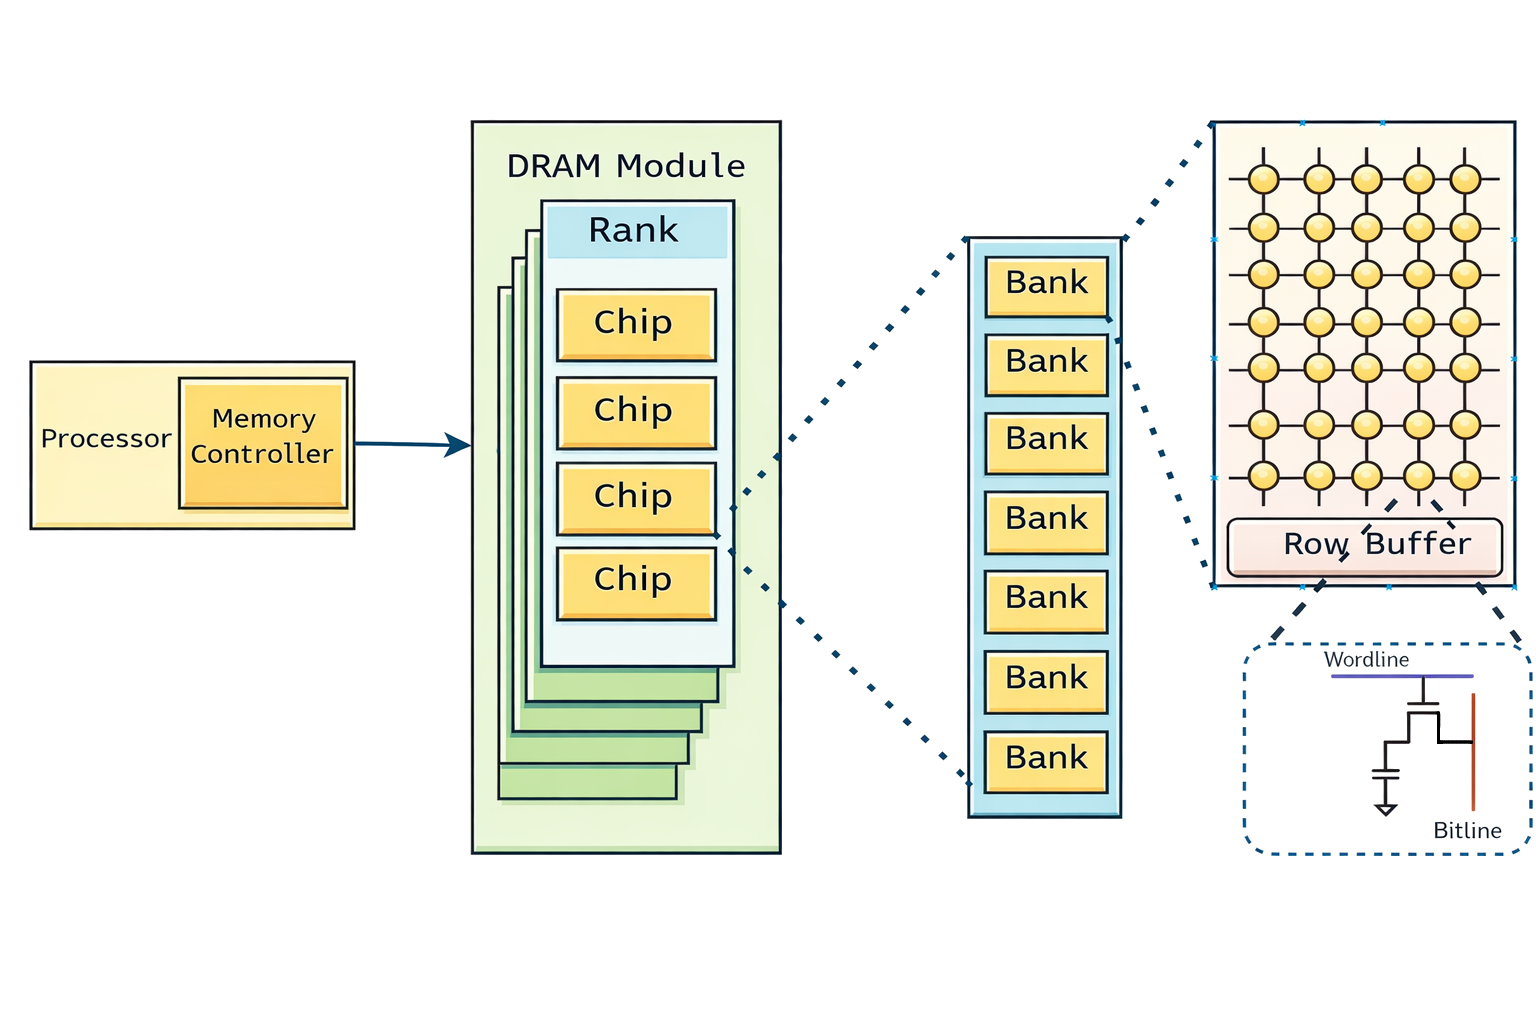
\includegraphics[width=\columnwidth]{drambanks_colored.png}
		\end{figure}
	\end{frame}
	
	\begin{frame}{What is RowHammer?}
		\begin{itemize}
			\item Dynamic Random-Access Memory (DRAM) is the short-term memory of a computer, storing data in densely packed rows.
			\item \textbf{The Attack:} Repeatedly accessing a row.
			\item \textbf{The Result:} Electrical interference, causing data bits in the adjacent "neighbor" rows to flip (e.g., a 0 becomes a 1).
			\item 
		\end{itemize}
	\end{frame}
	
	\begin{frame}{The Growing Threat: Why Do We Care Now?}
		\textbf{Shrinking Hardware, Growing Vulnerability}
		\begin{itemize}
			\item As technology advances, memory chips are packed with more data in physically smaller spaces[cite: 6, 99].
			\item Because the rows are closer together, it takes fewer "hammer strikes" to cause a bit-flip[cite: 98].
			\item In modern devices, the threshold to cause corruption has dropped drastically (down to 10k-20k activations), making the attack much easier to execute[cite: 100, 101].
			\item Mitigations that worked five years ago are now failing[cite: 31].
		\end{itemize}
	\end{frame}
	
	\begin{frame}{My Research Process}
		\textbf{Mapping the Defense Landscape}
		\begin{itemize}
			\item \textbf{Goal:} To survey and classify the latest defenses (especially post-2023) against RowHammer[cite: 7].
			\item \textbf{Methodology:} 
			\begin{itemize}
				\item Reviewed cutting-edge studies across major databases (IEEE, ACM, Google Scholar)[cite: 19, 20].
				\item Categorized defenses into three distinct approaches: Refresh, Frequency, and Isolation[cite: 7, 135].
				\item Analyzed how each defense system fails and the trade-offs they force hardware designers to make[cite: 14, 137].
			\end{itemize}
		\end{itemize}
	\end{frame}
	
	\begin{frame}{Defense Approach 1: Refresh-Centric}
		\textbf{The Quick Fix: Refreshing the Victims}
		\begin{itemize}
			\item \textbf{How it works:} Before the "noisy neighbor" can successfully corrupt the data, the system quickly "refreshes" the victim rows to restore their electrical charge[cite: 97, 162].
			\item \textbf{The Trade-off:} Keeping track of which rows need refreshing requires complex tracking arrays[cite: 164].
			\item \textbf{The Flaw:} As attacks get faster, the system has to refresh constantly, causing a massive slowdown for normal computer operations[cite: 324].
			\item In some cases, the refreshing action itself can be hijacked by the attacker to cause further damage[cite: 328, 329].
		\end{itemize}
	\end{frame}
	
	\begin{frame}{Defense Approach 2: Frequency-Centric}
		\textbf{Stopping the Attacker}
		\begin{itemize}
			\item \textbf{How it works:} Instead of protecting the victim, this method acts as a speed limit. It detects when a row is being accessed suspiciously fast and throttles or blocks the attacker[cite: 215, 216].
			\item \textbf{The Trade-off:} The system has to accurately guess if the rapid access is an attack or just a normal, heavy-duty program[cite: 244].
			\item \textbf{The Flaw:} False alarms! Innocent programs can be slowed down significantly, potentially denying normal services to the user[cite: 244].
		\end{itemize}
	\end{frame}
	
	\begin{frame}{Defense Approach 3: Isolation-Centric}
		\textbf{Building Walls and Moving Houses}
		\begin{itemize}
			\item \textbf{How it works:} Breaks the physical closeness of the attacker and victim. It either constantly shuffles data around (remapping) or places empty "guard rows" between them as a buffer[cite: 246, 247].
			\item \textbf{The Trade-off:} Security comes at the cost of valuable space[cite: 272].
			\item \textbf{The Flaw:} Dedicating memory rows purely to act as "security guards" means users lose out on overall storage capacity[cite: 272]. It can also create fragmented, underutilized memory areas[cite: 257].
		\end{itemize}
	\end{frame}
	
	\begin{frame}{Blindspots: We Weren't Looking at the Whole Picture}
		\textbf{The Rules Are Changing}
		\begin{itemize}
			\item \textbf{RowPress:} A newer attack variant showed that bits can flip just by keeping a memory door \textit{open} for a long time, rather than repeatedly opening and closing it[cite: 311]. This breaks the fundamental assumption of most reactive defenses[cite: 315].
			\item \textbf{Timing Side-Channels:} Smart attackers can observe how long the defense mechanisms take to activate and use that timing data to steal secrets invisibly[cite: 342, 343].
		\end{itemize}
	\end{frame}
	
	\begin{frame}{Core Conclusion: The Impossible Trinity}
		\textbf{You Can't Have It All}
		\begin{itemize}
			\item My research concludes that current defenses are trapped in a trilemma[cite: 18].
			\item The industry currently lacks a single mitigation that achieves all three:
			\begin{enumerate}
				\item \textbf{Space-Efficiency:} Not wasting memory space (fails in Isolation approaches)[cite: 12, 337].
				\item \textbf{Low-Latency:} Operating quickly without system slowdowns (fails in Refresh/Frequency approaches)[cite: 12, 336].
				\item \textbf{Deterministic-Security:} Mathematically guaranteed protection against all variants[cite: 12].
			\end{enumerate}
		\end{itemize}
	\end{frame}
	
	\begin{frame}{Looking Forward}
		\begin{itemize}
			\item Future defenses cannot rely on a single approach; they must be hybrid solutions combining strengths from different methods[cite: 365].
			\item We must rethink our basic assumptions about memory disturbance, moving from reactive band-aids to proactive, foundational hardware security[cite: 351].
			\item The industry urgently needs a standardized evaluation framework to honestly compare how effective these mitigations truly are[cite: 353, 356].
		\end{itemize}
	\end{frame}
	
\end{document}